% REMEMBER: You must not plagiarise anything in your report. Be extremely careful.
\providecommand{\tightlist}{%
  \setlength{\itemsep}{0pt}\setlength{\parskip}{0pt}}

\documentclass{l4proj}

    
%
% put any additional packages here
%

\begin{document}

%==============================================================================
%% METADATA
\title{Visualization of Classical Graph Theory Problems}
\author{Fatma Al-Sayegh}
\date{22 March 2023}

\maketitle

%==============================================================================
%% ABSTRACT
\begin{abstract}
Formalism in mathematics gives the subject a structure and a level of
abstraction which makes it applicable to the most general of the situations.
Visualization of a concept on the other hand, restricts the theory to a
particular example, but it makes one to see a problem in a more concrete
pattern. It may also allow the learner to see the same problem in a new light. The
learner can then apply or extrapolate the learning to other instances of the problem. 

In this project an application to elucidate some classical problems in Graph
Theory by the way of visualization is developed. The methods of visualization
are animations and user interaction with such animations. These methods aim to help young students and self-learners as to get the first brush with the subject of Graph theory.

The details and experience of analysis, design, development, testing and
evaluation of the application is discussed in this report.

The web application can be reached following
\href{https://visualise-graph-problems-with-me.netlify.app/} {this} 
\href{https://visualise-graph-problems-with-me.netlify.app/} {URL:} \\
\href{https://visualise-graph-problems-with-me.netlify.app/} {https://visualise-graph-problems-with-me.netlify.app/}
.

\end{abstract}

\renewcommand{\abstractname}{Acknowledgements}
\begin{abstract}
 I would like to thank my supervisor Sofiat for giving me a wonderful
    opportunity to explore the topics of Graph Theory. Her constant support and
    guidance throughout the project was essential in building the app. I would
    also like to thank my father for encouraging, believing and supporting me
    constantly in both the good and bad days. Finaly, I would like to thank my
    friend Shrey for introducing me to the Elm programming language. This
    project would not have been possible without the the help, aid and advice
    of friends and family. 
\end{abstract}
%==============================================================================

% EDUCATION REUSE CONSENT FORM
% If you consent to your project being shown to future students for educational purposes
% then insert your name and the date below to  sign the education use form that appears in the front of the document. 
% You must explicitly give consent if you wish to do so.
% If you sign, your project may be included in the Hall of Fame if it scores particularly highly.
%
% Please note that you are under no obligation to sign 
% this declaration, but doing so would help future students.
%
\def\consentname {Fatma Al-Sayegh} % your full name
\def\consentdate {20 November 2022} % the date you agree
%
\educationalconsent


%==============================================================================
\tableofcontents

%==============================================================================
%% Notes on formatting
%==============================================================================
% The first page, abstract and table of contents are numbered using Roman numerals and are not
% included in the page count. 
%
% From now on pages are numbered
% using Arabic numerals. Therefore, immediately after the first call to \chapter we need the call
% \pagenumbering{arabic} and this should be called once only in the document. 
%
% The first Chapter should then be on page 1. You are allowed 40 pages for a 40 credit project and 20 pages for a 
% 20 credit report. This includes everything numbered in Arabic numerals (excluding front matter) up
% to but excluding the appendices and bibliography.
%
% You must not alter text size (it is currently 10pt) or alter margins or spacing.
%
%
%==================================================================================================================================
%
% IMPORTANT
% The chapter headings here are **suggestions**. You don't have to follow this model if
% it doesn't fit your project. Every project should have an introduction and conclusion,
% however. 
%
%==================================================================================================================================
\chapter{Introduction}

% reset page numbering. Don't remove this!
\pagenumbering{arabic} 
% Introduction

\section{Motivation}
There are various kinds of phenomenon in nature and concepts in computer science which can
be modeled as graphs. Graphs can be thought of as points (called vertices or
nodes) related to each other by edges. The points can be humans in a social
network, genes in a gene expression network, proteins and metabolites
interacting with each other in a cell, various living species in an ecology or
a food-web. The nature of relations between such objects can be causation,
interdependence, interaction, etc.  Neural Networks, both natural and
artificial are graphs too.  There is a new field emerging in computer science
and statistical mechanics called \emph{Complexity}, which promises to enlighten
us about phenomenon such as life, ecology, intelligence, society and economy.
Graphs stand as one of the fundamental tool to model and study such complexity.
See Chapter 1 of \cite{Gros2015}.

Reducing a real world problem to a graph may amount to loosing details but as
graph theory has developed a number of tools for analysis and insight, these
tools become available immediately for a well formed inquiry. Therefore once a
concept in Graph theory is learned then just like other concepts in Mathematics
such as integers or vectors etc, it can be applied in a variety of fields of
study.

Although the most dependable way to study Graph Theory should be mathematical
formalism to state the terms, definitions and theorems; visualization of such
concepts can act as a first stepping stone for the uninitiated. It can also act
as an aid for a practitioner to enrich his understanding or to view the same
concept the same concept in a different light.

Using a particular example to define a topic in mathematics may diminish it's
generality. But a particular instance of a topic can give a concrete confidence
to a student about his understanding of the topic in consideration. It is
expected that a concrete example can be extrapolated by a student's mind for a
variety of situations and also a general understanding.

\section{Aim}
The aim of this project is to create computer visualization of classical graph
theory problems. To that end graph theory problems which are important in the
field should be shortlisted along with searching and designing of simple
examples and user stories to elucidate the definition of such problems.
The method of elucidation should be animation, interactive tasks and textual
explanation on a modern front end web application. To achieve this, a program
should be written to represent graphs and conduct basic operations on them;
with functionality to spawn such graphs visually on screen and
animate them using basic kinematics.

Finally, the advice of peers in the field should be sought to evaluate the
application in terms of usability and learning impact.

\subsection{Link to the Application}
For the reader's reference the application can be visited following this
URL: \\
\href{https://visualise-graph-problems-with-me.netlify.app/} {https://visualise-graph-problems-with-me.netlify.app/}.
%This project will take a route which is not taken often in terms of the
%programming paradigm it will employ. The program will be written in Elm, a
%functional programming language which makes the logic and implementation for
%the size of the project readable, reasonable and manageable.


% Elaborate about what are problems in Graph Theory.

% History of Graph Theory Problems?

% Survey of Graph Theory Problems?

% Survery of Applications of Graph Theory Problems?

% 


%\begin{enumerate}
%\item Graph Theory What?
%\item Why? Applications?
%\item How? History?
%\end{enumerate}
%
%\section{Motivation}

%==================================================================================================================================
\chapter{Background}
%Background

This chapter discusses concepts which are essential to understand the
forthcoming chapters in this report. It starts out by litrature review
discussing the books and research papers refered and consulted for this
project.Then it goes onto discuss Graph Theory definitions and it's classical
problems, which are useful to understand their implementation in the app.
Discussion of prior work on visualization of computer science topics which have
an influence over this project is also an part of research.

\section{Literature Review}
The books and the research papers which were referred to for this project range
from theoretical texts on Graph Theory, to Programming books on functional
programming and the functional programming language for web front end called
Elm.

\subsection{Graph Theory and Algorithms Literature}
Parts of the following literature was used to get familiar with the
basics of graph theory, some basic definitions and theorems and also
explanation of some classical graph theory problems. This literature
also played a role in shortlisting the graph theory problems which  
were chosen for the purpose of this project.
\subsubsection{Networks: An Introduction.}
This book was consulted for definitions, explanations and understanding of
basics of Graph Theory and it's problems. It discusses the mathematical and
computer science perspectives of the subject in dedicated sections. See \cite{Newman10}.
\subsubsection{Algorithm Design.}
This book lent the description and the example of \emph{Tree-width} problem
incorporated for an animation in the application.  See \autoref{explanation:
treewidth} for the explanation of the topic. In general, this book covers most
kinds of data structures and and has excellent portion on mathematical and
computer science aspect of Graph theory. See \cite{KleinbergTardos06}.

\subsection{Functional Programming and Elm Programming Literature}
In this section, literature covering functional programming and in particular
Elm programming language which were helpful in this project is reviewed.

\subsubsection{Why Functional Programming Matters.}
This paper is a terse tutorial using a Haskell like programming language called
Miranda, expositing the power of functional and modular thinking to glue
functions together to create and manipulate data structures like lists and
trees. It also discusses recurring patterns in programming and their
abstraction in form of higher order functions such as map, filter, and the
folds. In a steep learning curve it goes onto discuss some advanced concepts
in Artificial Intelligence. See \cite{Hughes89}.

\subsubsection{Elm in Action.}
This book can be used as a step by step tutorial introduction to the Elm
language and it's application in creating real world web apps. It starts with
small applications and gradually moves to the art of managing projects of
considerable size. It acts as a bridge between functional programming and
front-end design; it also dwells into front-end design recipies like how to
implement a single page application. See \cite{feldman2020elm}.

\subsection{Aesthetics}
\subsubsection{The Beauty of Simplicity.}
This paper provides arguments for how optimal simplicity, minimalism and
intuitiveness makes a user interface more usable and trustable. This paper was
the inspiration for keeping the website simple with the minimum of complicated
control and features. See \cite{Karvonen2000}.

\section{Discussion of Classical Graph Theory Problems}
This section formally discusses the concepts of Graph theory which are
elucidated visually in the application. If you are already familiar of the
topics discussed in this chapter then by all means skip over.  If not, then
it's recommended to go through the section as the material discussed here is
essential to understand the discussion in the further chapters.  The
forthcoming chapters will refer to the subsections here for definitions and
explanations.

\subsection{Definitions}
\label{graphtheory: definitions}
A \emph{Graph} $\boldsymbol{G}$, can be understood as a collection of vertices which are
connected to each other by edges.  A \emph{Vertex} $\boldsymbol{v}$ can be understood as a
point and an \emph{Edge} $\boldsymbol{e}$ is a pair of vertices.  The \emph{set of all the vertices}
in a graph $G$ is represented as $\boldsymbol{V(G)}$ and the \emph{set of all the
edges} in $G$ is represented as $\boldsymbol{E(G)}$.

For a vertex $v$, it's \emph{degree} $\boldsymbol{deg(v)}$ is the number of edges
connected to it.  An \emph{isolated vertex} $v$ is such that $deg(v) = 0$. An
\emph{end vertex} is a vertex $w$ such that $deg(w) = 1$.  Two vertices are
\emph{adjacent} to each other if there is an edge connects them.

A \emph{bipartite} graph, is a graph $G$ such that it's vertices $V(G)$ can
be split into two disjoint sets $A$ and $B$ such that each edge of $G$ joins a
vertex of $A$ and a vertex of $B$. See \cite{Newman10}.


\subsection{Graph Isomporphism}
Two graphs $G_1$ and $G_2$ are isomorphic if there is a one to one correspondence
between the vertices of $G_1$ and $G_2$ such that the number of edges between any
two vertices in $G_1$ is equal to the number of edges joining the corresponding
vertices of $G_2$.  Given two graphs, detecting if the graphs are Isomorphic is
a problem to solve as the graphs may appear to be different in appearance and
in the labeling of the nodes and edges. See \cite{Newman10}.

\subsubsection{Application}
The graph isomorphism problem finds application in the field of bioinformatics
for finding network motifs (sub-graphs isomorphic to an input pattern) in a
larger biological network. A network motif is a recurring pattern of connection
of vertices in a large graph signifying their evolutionary selection over
random patterns. See \cite{Bonnici2013}.

\subsection{Max K Cut}
A maximum cut, is partioning the vertices of a graph in two groups such that
the number of edges between these two groups is maximum. In a weighted graph,
where the edges are weighted, the weights of the edges are also taken into
consideration.  A maximum k-cut, is generalized version of maximum cut, where
the graph is partitioned into k subsets, such that the number of edges between
these groups is maximized.

It is important to note that a bipartite graph (refer to the Definitions
section above) is a trivial example of Max Cut there are no edges among the
vertices of a set $A$ and no edges among the vertices of set B and all the edges
are from the vertices in set $A$ to vertices in set $B$.

\subsection{Graph Coloring}
It is an optimization problem where the objective is to assign to the vertices
of a graph a color such that no two adjacent vertices have the same color,
while keeping the number of colors employed to a minimum. Here a color can be
thought of just any symbol from a finite set of symbols.

\subsection{Minimum Vertex Cover}
Minimum Vertex cover of a graph is the minimum amount of vertices such that,
all the edges in the graph must have one of such vertices as at least one of
their endpoints. This is also a optimization problem in which the constraint is
that all the edges must be covered while keeping the number of vertices in the
set of Minimum Vertex Cover to the minimum.

\subsection{Tree Width}
\label{explanation: treewidth}
We will explain in two parts. First we will define what a tree decomposition of
a graph is. Then we will define tree width of the graph.

To decompose a Graph in a tree is to put nodes into sets called pieces, subject
to certain conditions.  The first condition is that all the vertices of $G$
should belong to at least one piece. Every edge of $G$, must be present in
at least one piece which contains both ends of the edge.  And finally, in the
tree decomposition, if there is a node $n$ present in a walk from a node $n1$
to $n2$, and if both $n1$ and $n2$ have a vertex $v$ in common, then the node
$n$ also contains that vertex $v$. 

Any graph can be decomposed into a tree. Trivially, a graph can be tree
decomposed by putting all of it's vertices in just one node. But it will not be
a very useful tree decomposition.  Therefore a good tree decomposition of a
tree is the one which has small pieces.  Tree width is defined as the size of
the biggest piece $V_t - 1$. The smaller the tree width the bigger the better
the tree decomposition. See \cite{KleinbergTardos06} in the bibliography.

\section{Prior Work}
This project takes subtle inspirations from some of the work which is available
on the internet as web applications for visualization of popular algorithms.
Although the works which are discussed in this section are focused on
understanding algorithmic solutions of computer science problems, the
visualization of graphs, trees and lists in these projects have been inspiring
for depiction of graphs and their animation in this project.

\subsection{Data Structure Visualizations}
\label{priorWork: datastrucvisu}
This tool was developed by David Galles, Associate Professor, University of San
Francisco. See \cite{Galles}, in the bibliography section.  It covers topics
from various categories of computer science problems such as Dynamic
Programming, Geometric Programming, Trees, Heaps, Graphs etc.

The design of the tool has several important features. The user has the
facility to define his own data-structures rather than they being predefined or
hard-coded. There are control buttons which allow the user to start pause and
restart the animations. There is a slider to tune the speed of the animation as
well.

There is a dearth of textual explanation of the algorithms while they run.
Perhaps, the main purpose of this tool is as a teaching aid such that the
teacher first explains the topic and uses the tool as a visual demonstration to
show his students the working of the algorithm on real datastructures.

\subsection{VisuAlgo}
\label{priorWork: visualgo}
This tool was developed by Dr. Steven Halim of National University of
Singapore. See \cite{HalimVisu} in the bibliography. It covers topics from the
subject of data structures and algorithms. Most relevant for this project are
the topics related to graph theory; which are Maximum Flow, Minimum Vertex
Cover, Traveling Salesman and Steiner Tree, although the emphasis is on
algorithmic solutions to the problems and not problem visualization which is
the emphasis of this project.

For most topics the user is able to construct his instances of datastructures.
Unlike Data Structure Visualization application mentioned in
\autoref{priorWork: datastrucvisu}, there is an ample amount of textual
information in terms of theory, tutorial and instructions. The explanation of
the topics is done in text blocks which appear at appropriate places in a slide
show like fashion. For organizing the textual information, it has drop down
content menu for easy access to various sections. Although, different positions
of the text blocks can be a little distracting. In this project, the text explanation
is given at one place.


\subsection{Algmatch}
\label{priorWork: algmatch}
This Web app was developed as a final year individual project dissertation for
by Liam Lau under the supervision of Sofiat Olaosebikan. The application
visualizes the matching algorithms such as Gale-Shapley Stable Matching and
Extended Gale-Shapley Stable Matching algorithms applied to stable marriage and
hospital/residents problem. See \cite{LiamApp} in the bibliography. The app
lends ideas about user friendliness and intuitive usage.

It has a panel which describes the algorithm steps while in an animation the
matching algorithm works on an instance of the problem.

Aesthetically, the most noteworthy features of the app are, playback and speed
controls which are as intuitive as media buttons on a media player and smooth
page transitions resulting in a pleasing user interaction.

%==================================================================================================================================
\chapter{Analysis/Requirements}
In this chapter, the scope of the project, the criterion of selection of the
problems in graph theory, the thinking behind choosing the methods of
elucidation of the selected topics will be discussed. Finally to conclude the analysis
the requirements of the project are stated.


\section{Scope of The Project}

Understanding a problem is a necessary first step in trying to solve it.
It also enables a student to abstract out a mathematical
problem from a real life scenario present in the fields of science and engineering.

This idea has guided this project to be restricted to one which helps a learner to
understand the problem itself. The solution, on the other hand, or suggesting an
algorithm to solve the problem, if required, is the second important step which
has been deliberately not touched upon to keep the scope of this project
clear, precise and limited.


\section{Criteria for Selection of Problems}

One of the most important criteria for selection of the problems for the project was
based upon the importance of the topic in the field of graph theory. There are
several text books in graph theory, which discuss various theorems and problems in
the subject.  There are a few problems which occur commonly and frequently in
them. The order of their inclusion in the text books is based logically.
Building the concepts from the basics to advanced. Therefore the problems
included in the project should represent all hardness levels.

Since imagining a graph theory problem is largely a visual exercise, there
was no dearth of problems which could offer themselves as a subject of an
interesting visualization. The additional criteria therefore for filtering the
candidate problems was based on whether they could be elucidated in the form of a
simple and meaningful example, employed for animation and user
interaction. The simplicity of the example doesn't in anyway imply
triviality of the problem. Indeed here the assumption is that a simple example
problem can make a student reach to the heart of the concept in it's generality
fairly quickly. From there on she can extrapolate the learning to more
complicated examples.

It is important to mention here that a survey among
peers in the field of software engineering and computer science was conducted to 
gather suggestions on the shortlisted topics and methods.
The data from the survey had a role in determining topics and the methods chosen.


\section{Methods of Elucidation}
As it has been discussed in the previous section that feasible methods of
elucidation/exposition played a prominent role in the selection of the problems
in the first place. These methods can be broadly classified as animations and
user interactions or a combination of both.

\subsection{Animation}
The visual medium has dimensions such as of color, position, shape and motion.
Generating them with a computer program, scenes can be created attracting the
users attention towards a particular aspect of it with the help of animations.
The scene in this project consists of a graph, which undergoes transformations
of color, shape and position to make a certain aspect of it emphasized for the
purpose of explaining a concept.  Animations are used in this project to make
problems like Graph Isomorphism, Max Cut, and Tree Width. For instance, the
example problem of Graph Isomorphism, was explained by morphing a graph to change
it's shape to acquire another radically different shape. It will be explained
later how it can be considered as a visual proof that the two graphs in the
scene are thus isomorphic.

\subsection{User Interaction}
Although animations go a long way in terms of having a user's mind involved in
the learning process they only offer a linear narrative. On the other hand,
user interaction with an animation not only makes the experience more
immersive, it also leads to a natural multiplicity of stories from a single
program. This happens as a human input results in a novel path from one state to
another in the program just like a video game.

\section{Technical Scope of The Project}

To achieve the above mentioned features
The program has data structures to hold graphs and
algorithms to visually and geometrically manipulate them. 

It's important to note here the program does not 
contain algorithms to solve the listed problems. As the
scope of the program was limited to the purposes of visualization and not
coding the algorithms which can solve instances of the mentioned problems.
Therefore in this project, although the data type of Graphs (Set of
Vertices and Set of Edges) and the associated functions, are quite general and
can support operations of various kinds, care is taken that we provide the
solution to the visualization program before hand to give enough information to
the various animations and user interactions.


\section{Requirements}
Based on synthesis of the above sections it is concluded that
there should be a web application written for the desktop browser with user interactive animations which elucidate the following
graph theory problems -

\begin{enumerate}
\item Graph Isomorphism
\item Max Cut
\item Graph Coloring
\item Minimum Vertex Cover
\item Tree Width
\end{enumerate}

And to achieve all this by programming the following items -

\begin{enumerate}
\item Data structures which represent vertices, edges and graphs.
\item Display the above entities as Scalar Vector Graphics on screen.
\item Translation and shape transformation of the graphs for animation.
\item Generation and handling of events triggered by user interaction with the elements in the animation for user interaction.
\item Display appropriate text in synchronization with the animations and user interaction.
\end{enumerate}

Doing so in a manner which fulfills the following subjective qualities -

\begin{enumerate}
\item Substantive learning impact
\item Ease of Use
\item Coherent Story telling
\item Pleasing Aesthetics
\end{enumerate}

And finally, evaluating the application with the help of the peers on parameters which can be broadly classified into the following categories -

\begin{enumerate}
\item Quality of Elucidation
\item User Experience 
\item Learning Impact
\end{enumerate}

%==================================================================================================================================
\chapter{Design}
% DESIGN

This document discusses the design choices made for the application and the
guiding principles behind such choices. It progresses to how a graph are
visually displayed and animated in the app without going in the technical
details of implementation. Finally, I shall discuss the intended experience of
the user while going through the various topics explained in the application.
We will also discuss the learning impact of each topic on the user as it forms an essential
aspect of overall design.

\section{Guiding Principles}

\subsection{Simplicity}
\label{design: simplicity}
For the purpose of elucidation of Mathematical concepts, which requires an
undivided attention of the learner, it was decided that the user interface must
have the minimum amount of clutter possible, without giving away the minimum
amount of functionality required. The learner should not get distracted by an
overpopulated user interface. Simplicity and elegance would also lead the user
to stay longer on the application without getting visually exhausted.
Furthermore the users on the web today are extremely goal driven and don't want any
obstruction between them and their goal. See \cite{Karvonen2000}.

\subsection{Intuitiveness}
The layout of the user interface should be such that it not only has utility,
but should also help communicate the intention of the designer about the usage
of the application. For example a play button, just like it was found on media
devices for decades, invites the user to kick-start an animation even without
going through the text which tells him to do so explicitly. The size and
placement of the play button on the page, therefore becomes important. Right
placement of user interactive elements guide the user through the story which
is intended to be told.

\subsection{Meaningfulness}
For a substantial learning impact, the elucidation of the topics must reach at
the heart of the topic. Furthermore they must have a story line which is
meaningful and coherent. The learning outcomes of the animation or a
user-interactive task must be well defined before an attempt is made to
implement them.

\section{Wire-frame and Navigation}
The web application is a \textbf{Single Page Application}. Where the navigation
from one topic to another occurs according to the user inputs. When the state
moves from one graph theory to another topic, the data on the screen, that is
the graphics and the text, change on the same page without changing the url.

The page is vertical divided into two parts, the left part of the page contains
an instance of an animation, the right contains explanation of the topic and
advice on how to interpret the animation along with navigation and control
buttons. 

The text in the explanation part of the page is dynamic in nature, if the
animation has facility of user interaction with it's elements, the
corresponding text on the right responds with advises on the state of affairs
and what the user should do next.

There is a navigation bar at the bottom of the page, with left and right
arrows, along with the names of the previous and the next topics, to hop from
one topic to another.


\section{Animation Panel} 
As mentioned in the preceding section, the left half of the page is for
graphics, which contains an animation, a user-interaction session or a
combination of both.  The animation contains one or more than one graphs. These
graphs undergo, according to needs of the topic in consideration
transformations of appearance and annotation.

\subsection{Visual representation of graphs} 
The graphs are represented as vertices and edges joining those vertices.
Although the geometrical placement of the vertices is of no consequence in the
subject of graph theory, for the purpose of visualization, vertices are
assigned a 2 dimensional position. The edges, don't contain attributes such as
length or positions of endpoints of a line segment, they are rather defined as
a relation between a pair of vertices.

\subsubsection{Appearance of Vertices} 

The vertices of graphs in the animations are color filled circles of the
same size save for certain exceptions. The color of the vertices have been
allotted by varying mostly the hue and keeping saturation and lightness
relatively same in the \textbf{HSL} (Hue Saturation Lightness) color space. The
vertices contain a name inside the circle as an integer. The names of vertices
were chosen as integers as it was assumed that such a representation would help
the developer and also the user to keep a track of them as order of integers
is understood better by humans.

When a particular vertex is needed to be shown differently than the rest then
it's size and color are displayed differently. For example, a user-selected
vertex in some of the animations are shown bigger and it's color changed to
golden. The gold color it was observed makes the vertex in consideration
stand out differently from other colors in the animation.

\subsubsection{Appearance of Edges}
Edges, although are defined very algebraically as a relationship between a pair
of vertices it gets drawn by referring to the positions of the related vertices
as a straight line segment white in color.

When an edge is supposed to shown differently than the rest of the edges, it's
width is increased and color changed to the same value of golden as a selected vertex.
Again it was found that this color and thickness, made the edge standout from the
rest of the edges and helped in showing it distinguished without being unpleasantly
distracting.

\section{Explanation Panel}
Whereas, the animation panel on the left page contains all the graphical
components of the topic elucidation.  The right half of the page is occupied by
the Explanation Panel. It contains the title of the problem being explained,
it's definition and instruction on how to go ahead with starting the animation
or user-interactive tasks.  It also contains control buttons for starting,
re-starting and pausing animations.  For user-interactive tasks it has buttons
to reset the task.

As the animation or a user-interactive task progresses the explanation panel
generates explanatory and instructive text.

\section{User Stories for Elucidation of Topics}

This section describes, what the user is intended to experience while
interacting with the individual topics in the application with a special
consideration towards learning impact and understandibility.

When the user opens the web application on a browser of her choice, the first
topic she sees is that of Graph Isomorphism. She may stay there to interact
with the example of the topic or navigate to other topics using navigation
buttons at the bottom to have a bird's eye view of other topics.

Each graph theory problem has it's own character and require a different
approach for elucidation. The following sections will explain these approaches
with their intended experience on the user with learning outcomes which may be
achieved.

The survey mentioned in the \autoref{section: selectionCriteria}, also gave
quite a few suggestions on different ways to elucidate the short listed topics.
The suggestions were very topic specific, and included various ideas such as
animations and games and the ability to construct user defined graphs etc. Some
of the suggestions could be included in the project, some could not be
accomodated as they did not fit the flow of narrative, while others while being
brilliant ideas, act as inspiration for future work due to constraints of time.

\subsection{Graph Isomorphism}
The user is presented with a graph on the left and textual explanation on the
right of the page.  The textual explanation portion of the page also has some
media buttons such as play/pause and reset to interact with the explanation.
The text explanation briefly defines graph isomorphism and advises the user to
press the play button.

\subsubsection{Animation:}
When the user presses the play button, a new graph emerges out of the old one
while the keeping the edges between any two vertices conserved. While keeping
the connectivity between the vertices intact, the graph transforms into a
completely new shape, almost giving a visual proof that the two graphs on the
screen are isomorphic to each other.

\subsubsection{User Interaction:}
After the two isomorphic graphs have separated from each other, the user is
advised in a text panel to choose a vertex by either hovering over a vertex or
pressing the corresponding number on the keyboard. Doing so, will change the
visual appearance of the selected vertex, the edges incident on the selected
vertex and the adjacent vertices to the selected vertex in both graphs.  The
selected vertex will be enlarged to a new radius and change its color from it's
original color to golden color making it stand apart from the rest of the
vertices.  The edges incident on the vertex will change their colors to the
same gold color.  The adjacent vertices to the selected vertex will form a
golden halo around them.  This color transformation will distinguish a kind of
a subset in the two displayed graphs. At this point of time, in the text panel
the user is pointed out that the selected vertex has the same number of edges
connecting to the same adjacent vertices in both the graphs.  The user is also
advised to inspect other vertices of the graphs and convince herself that each
vertex of the graph has the same adjacent vertices in both the isomorphic
counterparts.

\subsubsection{Learning Impact:}
The transformation of a graph into a radically different looking graph but
being essentially the same as far as the connectivity between the vertices go
acts as a visual proof that the graphs are isomorphic.  While individually
inspecting each vertex will re-confirm this idea to the user. After having
experienced the concept of graph isomorphism in this way it is assumed that the
concept and definition of the term would be clear to her.


\subsection{Max k Cut}

Max Cut has two animations one after the other.  The first animation is about
Max 2 Cut and the second is about Max 3 Cut.  It is assumed that the user will
extrapolate the concept of the general Max k Cut after understanding the first
two cases ($k=2$, $k=3$) and extrapolating it over greater values of k.  The
examples shown in the animations are a nearly bipartite and a tripartite graph
for $k=2$ and $k=3$ respectively.  A nearly bipartite and a tripartite graph is
used to elucidate the topic as it is easier for the user to visualize how the
two graphs can be segregated to sets of vertices such that the maximum number
of edges pass between such sets.

In both the cases of $k=2$ and $k=3$, the weight of all the edges is taken to
be equal to $1$. This decision has been taken as with $w=1$, the answers to
both the max cut problems are more visual than unequal weights.

\subsubsection{Max 2 Cut Animation:} 
It starts with an Original graph on the left and definition of Max K Cut and
Max 2 Cut on the right of the web page. The right part of the page also
contains media buttons to pause and play the animations. It also has a button
for switching from Max 2 Cut example, to Max 3 Cut example.  The Max 2 Cut
animation starts with a graph, which starts when the user presses the play
button. As the animation progresses a new graph emerges out of the original
one and translates towards right changing it's shape to segregate it's
vertices into two sets forming a Maximum 2 Cut. The two sets move vertically up
and down and increase the distance between themselves, revealing the
number of edges passing from one set to another which the user can intuitively
tell is greater than the number of edges between any other two sets
which may have been formed from the vertices of the graph.

The user is advised to put up a pre-defined horizontal line by pressing a
button in the explanation panel. The line is drawn between the two sets of
vertices.  The intersection points between the edges and the max cut line is
shown by blue dots. These user is advised to observe the number of intersection
points which tell the user the number of edges passing from one set to another.

\subsubsection{Max 3 Cut Animation:}
Just like the animation for Max 2 Cut, this animation is started by the user by
pressing the play button. The animation on the right starts with a tripartite
graph arranged in a circular form. As the animation progresses the graph gets
Divided into three sets of vertices in which the three sets translate in
directions which are set $120^{\circ}$ apart from each other. The graph
transforms from a circularly arranged one to a triangular form. The user can
draw the Max 3 Cut lines at any point in the progress of the animation.  These
are three lines separating each set from the rest of the graph, with points of
intersection shown in blue showing the number of edges passing from one set to
the rest of the sets.

\subsubsection{Learning Impact:}
Although the examples in the Max 2 Cut and Max 3 Cut can be seen as simple ones
as the first one was nearly a bipartite graph and the second one was a
tripartite graph, they do a good job at defining the problem well. 
Not just that such visualization explains the problem well it also may act
as artwork especially in the case of Max 3 Cut, which may inspire an
imaginative student to want to investigate the subject further.


\subsection{Graph Coloring}
\subsubsection{User Interaction:}
A user-interactive task was chosen for explaining Graph Coloring as the nature
of the problem lends naturally for such.  The user is presented with a graph
which has all the vertices in color white.  On the explanation panel to the
right he is given the definition of the problem and advice on how to complete
the task.  

The task is to choose colors from a color palette of three colors namely red,
green and blue, and color vertices in the graph such that no two adjacent
vertices have the same color. Whenever the user colors two or more adjacent
vertices the same color the text panel warns them to make amends. There is a
reset button in the explanation panel to un-color all the vertices to start all
over again if the user wants to start from the beginning.

The user is challenged to first challenged to color the graph successfully in
just two colors but as it would be soon clear to the user it can only be done
in three.

A user-interactive task was chosen for explaining Graph Coloring as the nature
of the problem lends naturally for such.

\subsubsection{Learning Impact:}
The user interactive task will help the student retain the meaning of the Graph
Coloring problem in their memory for a long period of time than just watching
an animation as a spectator.

\subsection{Minimum Vertex Cover}
\subsubsection{User Interaction:}
Minimum Vertex Cover, by the nature of the problem is chosen to be
elucidated by the help of a user-interactive task. The user is given a graph
along with explanation of he Minimum Vertex Cover problem. He is also explained
how to complete the task. The task is to select vertices successively either by
clicking them or pressing a number corresponding to the vertex of choice on the
keyboard.  When he selects the vertex, the selected vertex and all the edges
incident on it are displayed differently. He has to thus highlight all the
edges by selecting the minimum number of vertices in the graph.  If he has done
this task effectively then he would not choose more vertices than required to
cover all the edges in the graph. When the user covers all the edges by only
selecting four vertices, he is given a congratulatory message for having done
the task right. If he covers the graph by selecting more than four vertices
then he is advised to do the same in just four.

\subsubsection{Learning Impact:}
Just like Graph coloring, in the case of Minimum Vertex Cover too, it is
assumed that a user-interactive task is effective not just in explanation of a
topic but also, retention of the concept for a long period of time.

\subsection{Tree Width}
\subsubsection{Animation:}
The topic Tree Width is explained in a multi-part animation. The first part
begins with a graph in which the vertices are arranged in a circular pattern.
The circular form conceals a tree like structure which can be abstracted out of
the graph. 

The user while reading the explanation is instructed to press the 'forward`
button to move to the first part. The user hops from one part of the animation
to another by pressing this 'forward` button.  In the first part the graph
which was hitherto arranged in a circular pattern transforms into a regular
lattice like pattern. The tree-like pattern is more apparent in the new visual
form of the graph.  This is also pointed out in the explanation panel.  

The next part of the animation shows an example of a piece (a sub-graph)
containing three vertices against the backdrop of the graph. The significance
of pieces in the tree-width concept is discussed in the background chapter.
The piece is also represented by a blue dot at the centroid of the three
vertices. In the next part of the animation the whole of the graph is marked by
it's constituent pieces by blue dots. 

In the final part, the pieces form the nodes of a tree. The tree's edges
(branches) are colored in golden color to make it stand out from the graph in
the background. At this point, the definition of the tree width is given in
the explanation panel.

\subsubsection{Learning Impact:}
The user is expected to learn the concept of tree decomposition of a graph.
Also, by the help of animations, he will be inspired to learn abstract
thinking: how a \emph{form} of a tree can be derived out of an unassuming
typical graph.

%==================================================================================================================================
\chapter{Implementation}
% Implementation

\section{Front End Development with The Elm Programming Language}

The project is developed using the Functional Programming paradigm. This is a
paradigm which has been in development and practice since the days of infancy of
computer science. Functional programming is based on a form of computation
called lambda calculus proposed by Alonzo Church.

For most of the history of computing functional programming remained in the
ivory towers of universities for purposes of exploring theoretical computer
science and language research.

In the last decades however, programming languages such as Haskell and a few
dialects of LISP have escaped the ivory towers to find application in the
software industry.

In this section we will discuss, why functional programming was chosen as the
programming paradigm of choice. How the functional programming language called
Elm is used to write a well organized, maintainable, intuitive and
understandable code to produce a dynamic front end.

\subsection{Why Functional Programming?}
Functional programming, makes the programmer think in a different way than what
may be called imperative programming. In the functional paradigm, functions are
first class citizens, which can be mashed up together with each other, by
giving a function as input to another function, a function giving out another
function as an output, function composed of two functions dove-tailed to each
other, programming patterns being abstracted out as functions and so on.

For such Lego like usage of functions they must be dependable, such that for a
particular input a function will give a particular output just like
mathematical functions and has no business outside it's scope for side-effects.
With such confidence in the functions, they can be fitted with each other to
make them do complex computation.

\subsubsection{Separation of Concerns}
It may be asked that if functions don't have side effects, how do they print
output on the terminal or read file from the hard disk or accept inputs from a
user. Functional programming environments have a way of separating the pure
part of a program from the impure part, by introducing 'actions'. These
'actions' or side-effects are treated as a form of encapsulated data, which
can be manipulated by pure functions, and the environment makes changes to the
outside world by executing these actions.

Therefore the programmer has to himself a large part of the program where he
deals with just pure functions. This allows him to exploit the perfectness of
pure functional programming.

This separation of concerns of pure and impure code in the context of the Elm
programming language is discussed in the next section called the Elm
Architecture.

\subsection{The Elm Architecture}
The Elm Architecture is a pattern of writing Elm code for responsive web applications. 
The architecture separates the concerns of front-end development into the following categories:

\begin{enumerate}
\item Model
\item View
\item Update
\end{enumerate}

The Model is a data structure which holds the state of a program. This state is
used by the view function to render a webpage. The webpage, when rendered has
elements, which may trigger events, such as user inputs by the way of clicking
an HTML element. Such events are caught by the Elm runtime and sent to the update
function.  The update function takes these event messages and changes the
state. The changed state is then rendered by the view function to a modified
page.  Therefore, the Model is changed by the update function, whereas it is
used by the view function to render a webpage according to a formula set by the
programmer.

The events described above are called messages in the Elm way of naming things. For this particular
application they are defined as an Algebraic Data Type as:

\begin{lstlisting}[language=elm]
type Msg
    = TimeDelta Float
    | HoverOver Int
    | MouseOut Int
    | VertexClicked Int
    | AnimationToggle
    | AnimationStartOver
    | ToggleVertexStatus Int
    | NextTopic
    | PreviousTopic
    | MaxCutLine
    | ColoringSelectColor Color
    | VertexNonColor
    | NextAnimation 
    | PreviousTreeWidthAnimation
    | ToggleHelpStatus
    | Other
\end{lstlisting}
The messages are not just generated by user interaction with this application, they are 
are also generated by the animation clock as well as can be seen in the first data constructor of the type Msg.

\section{Implementation of Graphs}
Inside the program, a graph exists as data structure which contains a list of
vertices and a list of edges. The vertex which is a data type defined
separately consists of a name (which is an integer), a color, a 2D position (it
is actually implemented using a 3D vector, with z is always kept at zero).  An
edge on the other hand is defined as a combination of two vertices. Such Graphs
are present in the Model in and are used by the view function to be drawn as
SVG.

\subsection{Grid}
In the program a Grid is a list of 3D vectors, which can be taken in by certain
functions to make graphs or change shapes of graphs.  A list of Vertices,
therefore can be formed by zipping together lists of names, colors and a grid.
There are functions, especially for implementing animations, which takes two
grids and outputs a grid which is geometrically in between the two grids.

\subsection{Using Linear algebra to Initialize Grids}
Linear algebra, in particular manipulation of vectors using Matrices has been
used to create interesting grids for the placement of vertices in the scene.
This includes rotation, scaling and translation of vectors to from polygonal
patterns. Functions were created to form polygon with $n$ geometric vertices
which prove very handy in producing grids for various geometries like
the one seen in Graph Ismoporphism and Max k Cut examples.

As a small example, here is a functional programming code to find the centroid
of of three position vectors. You can observe how first two vectors are added
on line 1, and then it is pipelined to addition with a third vector, which is
in turn pipelined to being scaled by $0.33$ (divided by $3.0$). This could have
been achieved in a single line of code, but Elm reserves operators like $+$,
$-$, $*$ for only numbers and they can't be overloaded to work for vectors.

\begin{lstlisting}[language=elm]
Math.Vector3.add v1.pos v2.pos
|> Math.Vector3.add v3.pos
|> Math.Vector3.scale 0.333
\end{lstlisting}

\subsection{Implementing Colors}
To have a list of neighboring colors acting as a color palette we work on the Hue Saturation Lightness
color space (HSl), mostly varying the hue
just pass a
region in the spectrum of hues (First, Second or Third) and the number of
colors needed as an Integer. On a scale from $0.00$ to $1.00$, the first region will produce hues ranging from $0.00$ to $0.33$,
the second producing it from $0.33$ to $0.66$ and the third producing it between $0.66$ to $1.00$.


\subsection{Edges}
Edges are defined as a combination of two vertices. Since they are drawn as a
straight line segment between the positions of the two vertices, they do not require
positional data associated explicitly for them. It is drawn out from the vertices,
they contain.


\section{Implementation of Animations}
In this section, it will be explained how various animations in the
application are implemented. Though there are minor differences between animations
for one topic to another, they follow a common pattern. The common pattern is
this that events are generated by a quasi-regular clock. These events trigger
the update function which transforms the current state of the program and
changes the position of certain abstract entities. The view function while
redrawing these entities takes the position information from the updated model
to draw them as SVG (Scalable Vector Graphics).

\subsection{Morphing Geometry of a Graph}
In some of the animations in the application, the graph changes it's geometry to
visually look different than the original. This is accomplished by a function which takes a graph
and a grid and moves the graph incrementally towards the grid with every tick
of the animation clock.  The function calculates the displacement vector
between a vertex and the respective final position given in the grid and finds
a new position along the direction of the displacement vector.

\subsection{Re-formation of the Graphs}
At each tick of the animation clock the graph under transformation, is built
again, with vertices having the same name and color as the original but new
positions. The edges need to be re-constructed again as the vertex positions
have been renewed. This is something which is expected in the functional
programming paradigm where nothing is changed in place and new data structures
are created with application of a function. This is true not just for
animations, it is true for user-interaction or anything which requires visual
(Geometric or Color) modification of the graph.


%==================================================================================================================================
\chapter{Evaluation and Testing} 
% Evaluation

\section{Evaluation}

An application such as this one, which aims to explain mathematical or
scientific concepts based on primarily animations and tasks must be evaluated
on two major aspects . The first aspect being user interaction and user
experience (UI/UX). The second one being the learning effectiveness.


The evaluation of the application was done on the basis of feedback from peers
mainly in the field of computer science and mathematics. There were two surveys
conducted, the first was unsupervised and anonymous. The second survey was
supervised in which the participants were interviewed while they were
experiencing the application.

\subsection{Unsupervised Survey}
The unsupervised survey was conducted among peers mainly in the field of
computer science, mathematics and education. The participants were given the
URL of the application and an online feedback form. See \autoref{links:
unsupervised} for the summary. The users were asked to visit the application
and answer a questionnaire.

Although the survey was anonymous, i.e. the names of the participants remained
unknown, but details such as their academic qualification and familiarity with
the subject of graph theory were obtained to put the responses in context.

The participants consisted of eleven PhDs, eight of which belonged to the field
of computer science. There were four participants with master's degree all of
whom belonged to computer science field. There were nine undergraduates mainly
from the field of computer science and engineering.

Among the eight PhDs in computer science, six mentioned that they have done
research in the field of graph theory, while the remaining two mentioned that
they had a course either exclusively on the subject or a wider field.
Therefore the feedback on the application brought a substantive quantity and
quality of opinions, criticism and even some praise.

The feedback ranged from opinions on UI/UX to 
opinions on effectiveness of a particular topic.


\subsection{Supervised Survey}
The supervised survey consisted of the same questions the as unsupervised
survey. See \autoref{links: supervised} for the summary. Though, unlike the
former survey the web application was visited by the participants by sharing
their computer screen. The participants unlike the unsupervised survey belonged
to a variety of education backgrounds like humanities, sciences and other
fields. Therefore the participants were frequently assisted while understanding
the animations and attempting the quizzes and tasks.

This gave the opportunity to see closely how the users navigate the app and
which aspects of the UI and the learning material they find confusing.

The Unsupervised Survey indicated that this application may be usable by high
school and mid school students. Therefore a supervised survey with young
participants was also done to explore the reach of the application's
effectiveness in that age group. See \autoref{links: supervisedvids}. This was
done after appropriate consent from their parents.


\subsection{Evaluation of UI/UX}
The survey was divided into two sections. The first part dealt with the user interface
and experience aspect of the application. There was both praise and criticism
from the participants. Both were taken into consideration and analyzed
in this section.

\subsubsection{Praise for UI/UX:}
Positive feedback for the UI/UX include the following comments:

\begin{quote}
\emph{``Very fluid. I like the single-page-application feel, rather than
needing to reload different pages.''}
\end{quote}

\vspace{0.06 in}
\begin{quote}
\emph{``The visuals and animation were pleasant. Quite easy to navigate.''}
\end{quote}

\vspace{0.06 in}
\begin{quote}
\emph{``.. it was intuitive and clear how to
interact with the application.''}
\end{quote}


The first \emph{quote} about the application being a single page application
(SPA) underlines an important aspect of the UX of the application.  It removes
distractions in the users learning experience. This is unlike ordinary
applications which while loading a new page briefly shows a white screen even
on fast connections.


\subsubsection{Criticism of UI/UX:}
There was constructive criticism of the UI/UX of the application as well.
Most of these criticisms were actionable while one criticism, given the
constraints put by the requirement of the topics was not.

\begin{quote}
\emph{``One thing I found a bit frustrating was the varying levels and styles of
interactivity between topics, such as clicking the cutline for max cut .. ''}
\end{quote}

\vspace{0.06 in}

\begin{quote}
\emph{``Maybe the topic words could be clickable to make navigation easier.''}
\end{quote}

\vspace{0.06 in}
\begin{quote}
\emph{``There are occasional spelling errors that
   could be corrected ..'' }
\end{quote}

The first criticism in the list above points out that the different topics had
different styles for interactivity.  Although, it is agreed that all the pages
should have consistency in the number and nature of interactive buttons
but the different demands of each topic made it difficult. For example the max
cut page has a cut-line button and others don't. This was unavoidable.
However, it is understood well that a variation in button layout and
functionality is potentially quite distracting. Perhaps, in a future iteration
of the application a drawer of tools which slides out and in can be made for
each page, though it may have it's own drawbacks in terms of visibility and
accessibility.

However most criticism of the UI/UX like clickable names on the navigation bar
were actionable.  For example, the users tend to click the words on the
navigation bar. Change in the implementation was made for the same. For
spelling errors in the explanation panel, they were combed out and corrected.


\subsection{Evaluation of Learning Effectiveness}
In general, from the feedback of the respondents, it could be gathered
that the application in learning effectiveness.

\subsubsection{Most Effective Topic:}
To obtain what the respondents think about the learning effectiveness of the
application they were asked which topic in the app did they find most effective
for learning. The answers ranged over all the topics. This indicates that every
topic had something to impress the respondents in terms of learning efficacy.


The respondents who are familiar with the field of graph theory mentioned
\emph{Tree Width}, and \emph{Max k Cut} the most. Although they mentioned rest
of the topics at least once. The two topics made to the top spot as they are
two most difficult topics to understand.

They were also asked about the least effective topic and the reason of their choice. 
This revealed some of the weaknesses in topic explanation. Again Tree width
faced the most criticism for lack of clarity in the explanation panel. 

\subsubsection{Graph Isomorphism:}
Graph Isomorphism was mentioned in the feedback positively for having both an
animation and a quiz. The animation was appreciated for having the
functionality in which, when a user hovers over vertices and the vertices and
the edges light up. 

However, there was a suggestion for the quiz 
that it would be nice if do a similar ``hovering functionality'' over the
vertices because the quiz was more difficult without it.

\subsubsection{Max k Cut:}
This was one of the most mentioned topic in the survey in a positive way,
perhaps because the difficulty in understanding it's definition. The cut-line
functionality has been praised by multiple respondents. Here are a few
comments on that from the respondents.

\begin{quote}
\emph{``Thought that max k cut was very well explained - the use of cutlines is
rather nice.''}
\end{quote}

\begin{quote}
\emph{``I love the way the graph transforms then you add the cutlines it was
creative.''}
\end{quote}

\subsubsection{Graph Coloring:}
The topic received mentions for the user interactive task. Perhaps, user
interaction is much favored way of learning than a passive animation.
It was most praised by the respondents who were not much familiar with
the field of Graph Theory. It should be so because it is a relatively easy
topic to understand compared to the other topics.

\subsubsection{Vertex Cover:}
Just like graph coloring, vertex cover found mention in the most effective topic for 
containing a user interactive task.

\subsubsection{Tree Width:}
Tree width was in the special focus of the respondents who are researchers in
the field.  Tree width received both praise and criticism. It received praise
for being at a different level of difficulty from the rest of the topics.

\begin{quote}
\emph{``
Tree Width is a hard problem to understand , you
have chosen an extraordinary way in visualising and explaining this
problem, made it seem simple and easy to learn.''}
\end{quote}

Identification of the pieces and decomposition was pointed out by various
respondents who are specialist in the field as significant in understanding the
topic. For example the following comments point the same out.

\begin{quote}
\emph{``
Tree width due to identification of blocks
''}
\end{quote}
\begin{quote}
\emph{``
I liked the pieces and decomposition .
I finally managed to start understanding Tree Width!''}
\end{quote}

Credit should be given to the book \cite{KleinbergTardos06} which lent a very
clear example of tree width which was adopted for the animation for this topic.

Tree width also received some constructive \textbf{criticism}. There was
ambiguity in the explanation of the possible tree decompositions of a graph and
possible tree widths corresponding to such decompositions. Here the emphasis
should be given to the word \emph{possible} which was not put at the appropriate
place in the explanation of the topic in the app. This was pointed out
by two respondents who are experts in the field. 

\begin{quote}
\emph{``
Treewidth wasn't very clear, unfortunately - I think it wasn't clear that the
treewidth of a graph is the smallest maximum bag size - 1 across all tree
decompositions. So it seems like a graph can have multiple different
treewidths, when it actually has multiple possible widths based on tree
decompositions, then a treewidth that doesn't depend on which tree
decomposition you use....''}
\end{quote}
\begin{quote}
\emph{``
Tree Width was my favourite maybe
you can try choosing better choice of words in the `explanation panel'  such as
`possible width decomposition'.''}
\end{quote}

Following their advice, a few more slides and the text on the animation panel
was changed so that the concept of tree width is clearly and correctly stated
removing ambiguities in the definition.


\subsection{Extra Feedback from the Respondents}
The application was commended for being clear and colorful and being
potentially extensible to other concepts of graph theory by most participants.
There were a few suggestions for extending the functionality such as:
\begin{enumerate}
\item Custom user graphs.
\item Detail on algorithms to compute these problems like vertex covers.
\item Animations showing non-optimal solutions.
\end{enumerate}


\subsection{Limitations}

The application has several fundamental limitaions some of which are pointed
out in the survey by the participants. Others are have been deduced
independently.

\subsubsection{Absence of Algorithmic Solutions:}
Since the objective of the application was to define and state the problems
clearly and not to solve them algorithmically, the explanation of algorithms to
solve the problems have been steered clear of. This limitation in the scope of
the project remains a limitation of the application.

\subsubsection{Easy Examples:}
The examples used to explain the topics are simple. For instance, the example
chosen to explain the max 3 cut problem was a tripartite graph.  It's solution
is trivial. These examples were chosen to clarify the definitions of the
problems, even though complicated examples could have given an uninitiated user
a flavor of complexity and hardness of the problems.

\subsubsection{Absence of Custom User Graphs Functionality:}
There are web applications on the internet, which allow the user to instantiate
their own graphs, with user instantiated vertices and edges. Although such
functionality has been avoided as the application's objective is to clarify the
definition of the problems. For this purpose in the application there are only
concrete examples which lend themselves to easy explanation of the problem at
the hand. However if in the future, algorithmic solutions to such problems, is
also included, then functionality of defining custom graphs can be added.

\section{Testing}
Automation of testing for this project was done by using a mix of Property
based Testing and Unit Testing. Both paradigms of testing can be implemented
for Elm projects using the library called \emph{elm-test} and a cli-tool which
goes by the same name. Writing test files in Elm is the same as writing any
other program. The test functions can generate input test cases (specially in
the case of property based testing) and use boolean predicates to generate the
output in terms of $Pass$ or $Fail$.

\subsection{Property Based Testing}
Testing of components of Graph module was done using Property Based Testing (PBT).
This paradigm of testing was introduced for the first time for Haskell (a
functional programming language). It checks if the output of a function
satisfies certain prescribed properties. These properties are specified as
boolean predicates.

For example, a function which constructs a fully connected graph (a graph in
which all the vertices are connected to each other by one edge) with $n$
vertices, will form $n (n - 1) / 2$ edges. The number of edges of the output
graph are matched up against this mathematical reality. The function passed
the test against a vast number of auto generated inputs.

Similarly, a cyclical graph i.e one in which the vertices are connected in a
pattern such as this: A -- B -- C -- D -- A, with n vertices will have the
number of edges equal to $n$. A function which constructs such a graph can be
property based tested by comparing the number of edges it has with the number
of vertices, which in this case should be equal. See \autoref{testing: pbtExamples}
for examples of testing functions and see \autoref{testing: results} for the results.

\subsection{Unit Testing}
Unit testing was done on for the functionality of graph animations and
functions responsible for navigation in the application against possible inputs
and reference outputs. See \autoref{testing: results} for the results.

\subsection{Manual System Testing}
The system was continuously tested manually during the development of the
project. Regardless, towards the end of the development a planned scheme for
interacting with the system for the black box testing of the application was
executed to search for unexpected behavior. See \autoref{appendix:
manualTesting} for the details of the test and results. The application's
behavior against all the tests was as expected.

\section{Verification of Satisfaction of Requirements}

\subsubsection{Verification of Development of Interactive Animations:}
The requirements mentioned in \autoref{requirements: requirements} have been
primarily satisfied by this application.  The application has covered all the
topics it had set out to achieve. As can be seen in the
\href{https://visualise-graph-problems-with-me.netlify.app/} {\textbf{application}}.



\subsubsection{Verification of Development of Data Structures and Functions:}
The data structures and the function to represent the graphs and it's elements
in the program; drawing of the graphs on screen; animating translation and
shape transformation of graphs; handling of events generated by elements in the
graph and explanation panel and synchronization of the explanation panel with
the state of the graphs was achieved as dictated by the requirements. The
code of the program can found in \autoref{links: repository}.
 

\subsubsection{Verification of Learning Impact:}
Although evaluating a learning method for it's effectiveness is a subjective
issue, the respondents of the evaluation survey have expressed their
satisfaction in the quality of the animations and tasks. Several have
commented that it could be a learning tool in reality.

\subsubsection{Verification of the Quality of User Experience:}
The respondents and the first users have evaluated UI/UX of the application as
simple and intuitive. The Single page application feel has been appreciated for
fluid and unobstructive. 

\subsubsection{Verification of Should Have Requirements:}
Fon satisfaction of \emph{Device Compatibility} requirement, the application has been
tested on various screen sizes of desktop computers, laptop computers, modile
devices and fits those screen sizes by properly placing the display and
explanation divisions.
For satisfaction of \emph{Pleasing Aesthetics}, see \emph{Verification of the Quality of
User Experience} in this section.
For satifaction of the \emph{Contribution Friendliness} requirement, the code
is published publically on GitHub and will invite public contribution
after the completion of the dissertation. See \autoref{links: repository}.  The
program is well modularized and new sections can be added to it by adding
another elm file for a new topic and making a few changes in $Main.elm$.

%==================================================================================================================================
\chapter{Conclusion}    
% Conclusion

\section{Reflections}

%\subsection{On Learning Impact}
%\subsection{On Problem Explanation}
%\subsection{}

\subsection{Experience on Project Management}
For a project of this size, well begun is half done. The majority of the work
must be completed should be done early. The concluding days of the project
should be reserved for evaluation, and feedback and subsequent changes.

The project, in retrospection was done in the several phases. The
\emph{first} phase which lasted a week was about how to spawn a page on a
Single Page Application and how to use vectors and matrices to position
elements of Scalable Vector Graphics. The \emph{second} phase was how to
implement graph, vertices and edge data-structures; achieving translation and
morphing animations and development of the graph isomorphism topic and making
it's explanation panel. The \emph{third} phase, which took almost a month was
to use the learning from the topic to implement rest of the topics and
refactoring the code in several modules.


Functional programming paradigm contributed in preserving sanity for managing
the size of the program. More reflection on this is in \autoref{reflection:
functional}. 

\subsection{Experience on the Evaluation of the Application}
It was observed that while gathering opinion and advice on usage of an
application, specially a kind which has a particular utility in terms of
education and learning; quality of advice is better than it's quantity. The most
valuable advice and opinions came from the research scholars and postgraduates
in the field of computer science who had either conducted research in the field
or had taken a semester course on it. Such advice was adopted and appropriate
changes were subsequently made.


\subsection{Experience of using Functional programming for Front End Programming} 
\label{reflection: functional}

Here is a reflection on the experience of using functional programming for this
project. This experience will also be compared to past experience in
programming in imperative languages.

A web app today is one of the primary means of human computer interaction
(HCI). To model something as complex as a HCI a programming paradigm which can
model this complexity efficiently is needed. 

An imperative programming language, however \emph{high-level} it might be, is
much closer to the Von-Nueman machine in terms of how a computer program is
reasoned about by the programmer. There is a tape and it has to be read one
step at a time. The programmer implements most of the logic in terms of control
mechanisms and less in terms of logic itself. Therefore the program becomes far
more complex than the actual complexity it has to represent. 

Functional programming on the other hand was much more efficient in modelling
the domain to be represented. It implemented logic more in terms of logic and
less in terms of control structures. Such that while reading the program one
mostly saw logic and not boiler-plate code.

Using Elm in representing the world inside the application and the signals
which are received from the outside was simple and elegant. The functional
\emph{type system} gave a structure for organizing, extending and refactoring
the project which continued to grow in size and complexity. The ease of
extending the application nudged the development style towards more of a
bottom-up style. Functionality of the animations were coded before pages, and
pages were done before the whole of the app.

While types made modelling the domain efficient. Functions made the rules of
physics in the web application explicit. Pattern matching on the inputs of the
functions was used extensively in the code to take logical decisions. Another
important method was pipeling the output of a function to the input of another
function. Reading a series of pipelined functions, was easy to reason with as
it seemed like data is being processed on an assembly line with functions
acting on it in turn.

%==================================================================================================================================
%
% 
%==================================================================================================================================
%  APPENDICES  

\begin{appendices}

\chapter{Links to External Resources}
% Important Links

\section{The Web Application}
\href{https://visualise-graph-problems-with-me.netlify.app/} 
{https://visualise-graph-problems-with-me.netlify.app/}

\section{Git Hub link of The Project Repository}
\label{links: repository}
Here is the Git Hub link for the Project. It consists of documentation, report and the
code of the Web Application.

\href{https://github.com/FatmaSayegh/Level4Report} {https://github.com/FatmaSayegh/Level4Report}

\section{Form for Feedback on Initial Concept}
\href{https://docs.google.com/forms/d/1MMN1H8YMCPlG9Modh5vv0Hy2ZHLsvvW769WPRKvuKF0/viewanalytics} {https://docs.google.com/forms/d/1MMN1H8YMCPlG9Modh5vv0Hy2ZHLsvvW769WPRKvuKF0/viewanalytics}

\section{Unsupervised Evaluation Survey Form}
\label{links: unsupervised}
\href{https://docs.google.com/forms/d/1G-RElMkFfn5TBZN5Os2lmySNeMe8DzWCH4nKqPKjRTw/viewanalytics} {https://docs.google.com/forms/d/1G-RElMkFfn5TBZN5Os2lmySNeMe8DzWCH4nKqPKjRTw/viewanalytics}

\section{Supervised Evaluation Survey Form}
\label{links: supervised}
\href{https://docs.google.com/forms/d/1LzBP-KeheT2cCgGcfkuarrLV47omhg7ei6WIQbdvx-8/viewanalytics} {https://docs.google.com/forms/d/1LzBP-KeheT2cCgGcfkuarrLV47omhg7ei6WIQbdvx-8/viewanalytics}

\section{Supervised Evaluation Videos}
\label{links: supervisedvids}
(Parental consent was taken while interviewing the minors and sharing the videos)

\chapter{Unit and Propery Based Testing Information}
% Testing info
\graphicspath{ {images/} }

\section{ Result of Running the Tests.}
\label{testing: results}
The unit and property based testing were done by running the cli command \emph{elm-test}.
This is a snapshot of the terminal.

\begin{figure}[!ht]
\centering
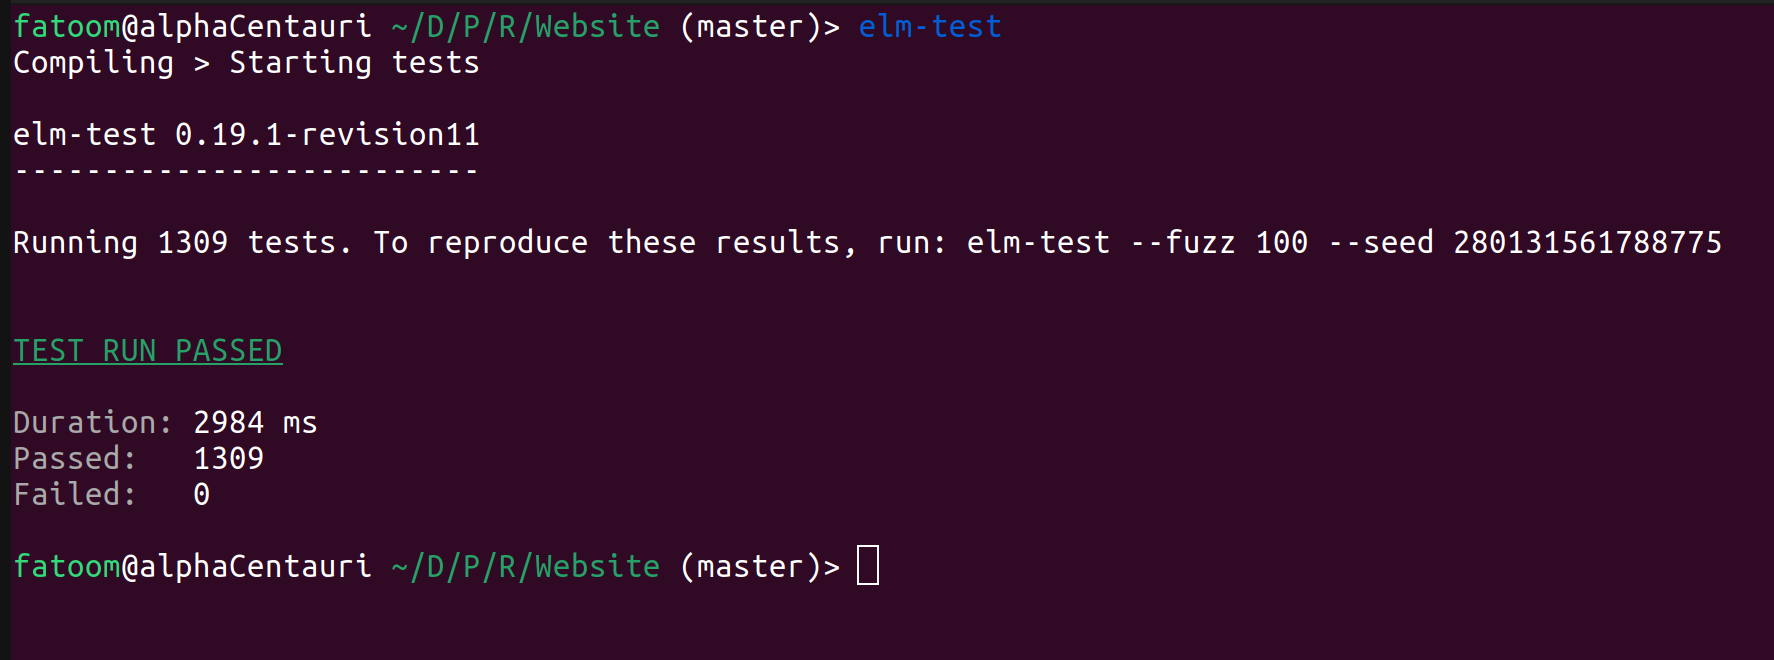
\includegraphics[width=4.70in]{testResultsSnap}
\caption{
        Results of unit and property based testing.
        }
\end{figure}

\section{Examples of Property Based Testing}
\label{testing: pbtExamples}
The first example checks if a fully connected graph is constructed well by
counting the number of edges which have been formed. The second example
generalizes this to test many types of graphs. Here also the number of edges
formed is compared against the mathematical number of edges which a particular
kind of graph should have.

\begin{lstlisting}[language=elm
                  , caption={
                  Property Based Testing of construction of a fully
                  connected graph.
                  }
                  ]
fullyConnectedGraphEdgeCountSuite : Test         
fullyConnectedGraphEdgeCountSuite =
   describe "fully connected graph edge count suite " <|
   let
      polySize =
         List.range 3 100
   in
   List.map
      fullyConnectedGraphEdgeCountTest         
      polySize

fullyConnectedGraphEdgeCountTest : Int -> Test         
fullyConnectedGraphEdgeCountTest n =
   let
      size = (vec3 100 100 0)

      pos = (vec3 100 100 0)

      graph =
         makeGraph
            (PolygonFullyConnected n)
            size
            pos
            0

      noOfEdges =
         graph.edges
         |> List.length

  in
  test ("fully connected graph edge count " ++ (String.fromInt n)) <|
   \_ ->
      Expect.equal 
         (( n * ( n - 1) )//2)
         noOfEdges
\label{listing: testA}
\end{lstlisting}

\begin{lstlisting}[language=elm
                  , caption={
                  Property Based Testing of construction 
                  graphs based on their type. For example,
                  the graph with a given number of vertices
                  should have the number of edges dependent on
                  the number of vertices.
                  }
                  ]
makeGraphNoVerticesSuite : Test
makeGraphNoVerticesSuite =
   describe "Checking if correct number of vertices is made correctly " <|
      let
         polygonSizes =
            List.range 3 200

         polygonCycles =
            List.map PolygonCycle polygonSizes

         fullyConnecteds =
            List.map PolygonFullyConnected polygonSizes

         dolls =
            List.map PolygonCycleDoll polygonSizes

         combinedGtypes =
            polygonCycles ++ fullyConnecteds ++ dolls
      in
      List.map
         makeGraphNoOfVerticesTest combinedGtypes

makeGraphNoOfVerticesTest : Gtype -> Test
makeGraphNoOfVerticesTest gtype =
      let
         sizeOfGraph =
            (vec3 150 150 0)

         positionOfGraph =
            (vec3 150 150 0)

         graph =
            makeGraph gtype positionOfGraph sizeOfGraph 0

         (expNoVer, gtypeStr) =
            case gtype of
               PolygonCycle n ->
                  (n, "Cycle")
               PolygonFullyConnected n ->
                  (n, "Fully Connected")
               PolygonCycleDoll n ->
                  (2*n, "Doll")
      in
      test 
         ("No. of vertices according to type of graph " 
            ++ String.fromInt expNoVer
            ++ gtypeStr)  <|
         \_ ->
            graph
            |> .vertices
            |> List.length
            |> Expect.equal expNoVer
\label{listing: testB}
\end{lstlisting}

\chapter{Manual System Testing}
% Manual System Testing Appendix
\label{appendix: manualTesting}
In this appendix, the details of the manual system tests and their resuls are
tabulated.
\section{Home Page Testing}
%\begin{center}
\begin{tabular}{ |p{1cm}|p{2cm}|p{4cm}|p{2cm}|p{2cm}| }
 \hline
 \textbf{Test Id} & \textbf{Test Case} & \textbf{Note} & \textbf{Expected} & \textbf{Actual} \\
 \hline
 \hline
 1 
 & URL of the home page works 
 & Typing the URL on the navigation bar of the browser loads the home page of the web app
 & Home page of the Web app loads 
 & As expected \\
 \hline
 2 
 & Home page button works 
 & Pressing the Home page button should not change the page shown on browser.
 & Home Page stays on the browser
 & As expected \\
 \hline
 3 
 & About Page button works 
 & Pressing the About Page button on the header bar puts the About Page on the browser
   with the relevant url on the navigation bar of the browser.
 & About page is displayed.
 & As expected. \\
 \hline
 4 
 & Title of the application is horizontally centered.
 & Title of the application is at the center of the page on different screen sizes.
 & Title of the screen size is at horizontally centered.
 & As expected. \\
 \hline
 5 
 & Proper display of icons of graph theory topics.
 & The two rows of icons are horizontally centered and contain minigraphs
 of corresponding topics.
 & Mini graphs appear in the icons and icons are aligned nicely.
 & As expected. \\
 \hline
 6 
 & Clicking on topic icons
 & Clicking on the topic icons should take the user to the relevant page. 
 & Clicking on the topic icons should take the user to the relevant page.
 & As expected. \\
 \hline
\end{tabular}
%\end{center}


\section{About Page Testing}
\begin{tabular}{ |p{1cm}|p{2cm}|p{4cm}|p{2cm}|p{2cm}| }
 \hline
 \textbf{Test Id} & \textbf{Test Case} & \textbf{Note} & \textbf{Expected} & \textbf{Actual} \\
 \hline
 1 
 & Elements appear at the intended positions.
 & All the elements appear at the right positions. The topic and description
 appears at the center and rest of the elements are left and right aligned
 alternatively and the page is scrollable.
 & All elements are at their respective positions.
 & As expected. \\
 \hline
\end{tabular}

\section{Header Bar Testing}
\begin{tabular}{ |p{1cm}|p{2cm}|p{4cm}|p{2cm}|p{2cm}| }
 \hline
 \textbf{Test Id} & \textbf{Test Case} & \textbf{Note} & \textbf{Expected} & \textbf{Actual} \\
 \hline
 1 
 & Header bar appears at the top of every page.
 & Header bar gives user the navigation options to go to the Home page (which has the contents)
   and the about page.
 & All the pages visited on the application must have the header bar.
 & As expected. \\
 \hline
 2 
 & Header bar stays at it's position.
 & Header bar stays at the top of the page, even if the rest of the page is scrolled.
 This must be true for all the pages on the application. 
 & All pages must have the header bar at top even if rest of the page is scrolled.
 & As expected. \\
 \hline
\end{tabular}


\section{Isomorphism Page Testing}
\begin{tabular}{ |p{1cm}|p{2cm}|p{4cm}|p{2cm}|p{2cm}| }
 \hline
 \textbf{Test Id} & \textbf{Test Case} & \textbf{Note} & \textbf{Expected} & \textbf{Actual} \\
 \hline
 1 
 & Url of Isomorphism Page Works. 
 & In an SPA ideally each page be independently reachable with it's own unique
   Url.
 & Typing Url of the isomorphism path conclatenated to the url of the app will load the
   isomorphism page 
 & As expected. \\
 \hline
 2 
 & All elements of the page are diplayed.
 & All the elements of the page, the display part, the explanation panel, along with the
   buttons are present on the page.
 & All intended elements page are present.
 & As expected. \\
 \hline
 3 
 & Animation is working for the first part of the Isomorphism topic.
 & At the press of the play button, the animation starts. When the press of pause button
   is pressed animation is paused. When the restart button is pressed, the animated graph
   moves to the initial position.
 & All intended function of the animation and the buttons are working as intended. 
 & As expected. \\
 \hline
 4 
 & Next Task button.
 & Pressing the next task button from the first animation in the Isomorphic topic 
   should take the user to the next task in Isomorphic topic.
 & The second task of the Isomorphism topic is displayed.
 & As expected. \\
 \hline
 5 
 & All elements of the task are displayed.
 & On the task section of the Isomporphic page being displayed, all elements of
   the page should appear at their respective positions.
 & All elements of the page are at their intended positons.
 & As expected. \\
 \hline
 6 
 & The quiz is functioning as intended. 
 & Functionality, of choosing the right option, pressing of the check button and
   resulting animation on the display panel and resulting change in explanation
   panel, even if the task is carried out by the user out of order should not
   lead to the application showing unexpected behaviour.
 & All intended function of the task and the buttons are working as intended. 
 & As expected. \\
 \hline
\end{tabular}

\section{Max k Cut Page Testing}
\begin{tabular}{ |p{1cm}|p{2cm}|p{4cm}|p{2cm}|p{2cm}| }
 \hline
 \textbf{Test Id} & \textbf{Test Case} & \textbf{Note} & \textbf{Expected} & \textbf{Actual} \\
 \hline
 1 
 & Url of Max k Cut Page Works. 
 & In an SPA ideally each page be independently reachable with it's own unique
   Url.
 & Typing Url of the Max-Cut path conclatenated to the url of the app will load the
   Max K Cut page. Showing the Max 2 Cut page of the topic.
 & As expected. \\
 \hline
 2 
 & All elements of the page are diplayed.
 & All the elements of the page, the display part, the explanation panel, along with the
   buttons are present on the page.
 & All intended elements page are present.
 & As expected. \\
 \hline
 3 
 & Animation is working for the first part of the Max k topic.
 & At the press of the play button, the animation starts. When the press of pause button
   is pressed animation is paused. When the restart button is pressed, the animated graph
   moves to the initial position. The cut-line button produces a cut line over the graph.
 & All intended function of the animation and the buttons are working as intended. 
 & As expected. \\
 \hline
 4 
 & Next Animation button.
 & Pressing the next animation button from the Max 2 Cut part of the topic 
   should take the user to the Max 3 cut topic and all the elments
   of that topic must be present at the right position.
 & Max 3 Cut topic is displayed on the browser.
 & As expected. \\
 \hline
 5 
 & Animation is working for the second part of the Max 3 topic.
 & At the press of the play button, the animation starts. When the press of pause button
   is pressed animation is paused. When the restart button is pressed, the animated graph
   moves to the initial position. The cut-line button produces a cut line over the graph.
 & All intended functions of the animation and the buttons are working as intended. 
 & As expected. \\
 \hline
\end{tabular}

\section{Graph colouring Page Testing}
\begin{tabular}{ |p{1cm}|p{2cm}|p{4cm}|p{2cm}|p{2cm}| }
 \hline
 \textbf{Test Id} & \textbf{Test Case} & \textbf{Note} & \textbf{Expected} & \textbf{Actual} \\
 \hline
 1 
 & Url of Graph colouring Page Works. 
 & Graph colouring page be independently reachable with it's own unique
   Url.
 & Typing Url of the Graph colouring path conclatenated to the url of the app will load the
   Graph colouring page.
 & As expected. \\
 \hline
 2 
 & All elements of the first graph colouring task are displayed.
 & On the task section of the graph page being displayed, all elements of
   the page should appear at their respective positions.
 & All elements of the page are at their intended positons.
 & As expected. \\
 \hline
 3 
 & The tasks are functioning as intended. 
 & Functionality, of picking up the right colour from the colour palette,
   colouring the vertex, diplay of edges with wrongly coloured vertices, diplay of
   appropriate text depending on the state of the task and the uncolour button
   even if the tasks are carried out by the user out of order should not lead to
   the application showing unexpected behaviour.
 & All intended function of the tasks and the buttons are working as intended. 
 & As expected. \\
 \hline
 4 
 & Next Task button.
 & Pressing the next task button from the first task
   should take the user to the second task.
 & Next Task is diplayed on the browser on the press of the relevant button.
 & As expected. \\
 \hline
\end{tabular}

\section{Vertex Cover Page Testing}
\begin{tabular}{ |p{1cm}|p{2cm}|p{4cm}|p{2cm}|p{2cm}| }
 \hline
 \textbf{Test Id} & \textbf{Test Case} & \textbf{Note} & \textbf{Expected} & \textbf{Actual} \\
 \hline
 1 
 & Url of Vertex Cover Page Works. 
 & Vertex Cover page be independently reachable with it's own unique
   Url.
 & Typing Url of the Vertex Cover path conclatenated to the url of the app will load the
   Vertex Cover page.
 & As expected. \\
 \hline
 2 
 & All elements of the first vertex cover task are displayed.
 & On the task section of the graph page being displayed, all elements of
   the page should appear at their respective positions.
 & All elements of the page are at their intended positons.
 & As expected. \\
 \hline
 3 
 & The tasks are functioning as intended. 
 & Functionality, of the task of selecting the vertices, and display of the
 edges incident on such edges, and appereance of corresponding text even if the
 tasks are carried out by the user out of order should not lead to the
 application showing unexpected behaviour.
 & All intended function of the tasks are working as intended. 
 & As expected. \\
 \hline
 4 
 & Next Task button.
 & Pressing the next task button from the first task
   should take the user to the second task.
 & Next Task is diplayed on the browser on the press of the relevant button.
 & As expected. \\
 \hline
\end{tabular}

\section{Tree Width}
\begin{tabular}{ |p{1cm}|p{2cm}|p{4cm}|p{2cm}|p{2cm}| }
 \hline
 \textbf{Test Id} & \textbf{Test Case} & \textbf{Note} & \textbf{Expected} & \textbf{Actual} \\
 \hline
 1 
 & Url of Tree Widht page works. 
 & Tree width must page be independently reachable with it's own unique
   Url.
 & Typing Url of the Max-Cut path conclatenated to the url of the app will load the
   Max K Cut page. Showing the Max 2 Cut page of the topic.
 & As expected. \\
 \hline
 2 
 & All elements of the page are diplayed.
 & All the elements of the page, the display part, the explanation panel, along with the
   buttons are present on the page.
 & All intended elements page are present.
 & As expected. \\
 \hline
 4 
 & Next Animation/Previous Animation buttons.
 & The next animation and previous animation buttons hop between the intended animations
   in series.
 & The Next and Previous Animation buttons work as intended.
 & As expected. \\
 \hline
 3 
 & The series of Animations are working.
 & The animations in the series occur in right order and each work as intended. 
   each is accompanied by the intended text in the explanation panel.
 & The animation and explanations work as intended.
 & As expected. \\
 \hline
\end{tabular}

\chapter{Ethics Form}

\begin{figure}[!ht]
\centering
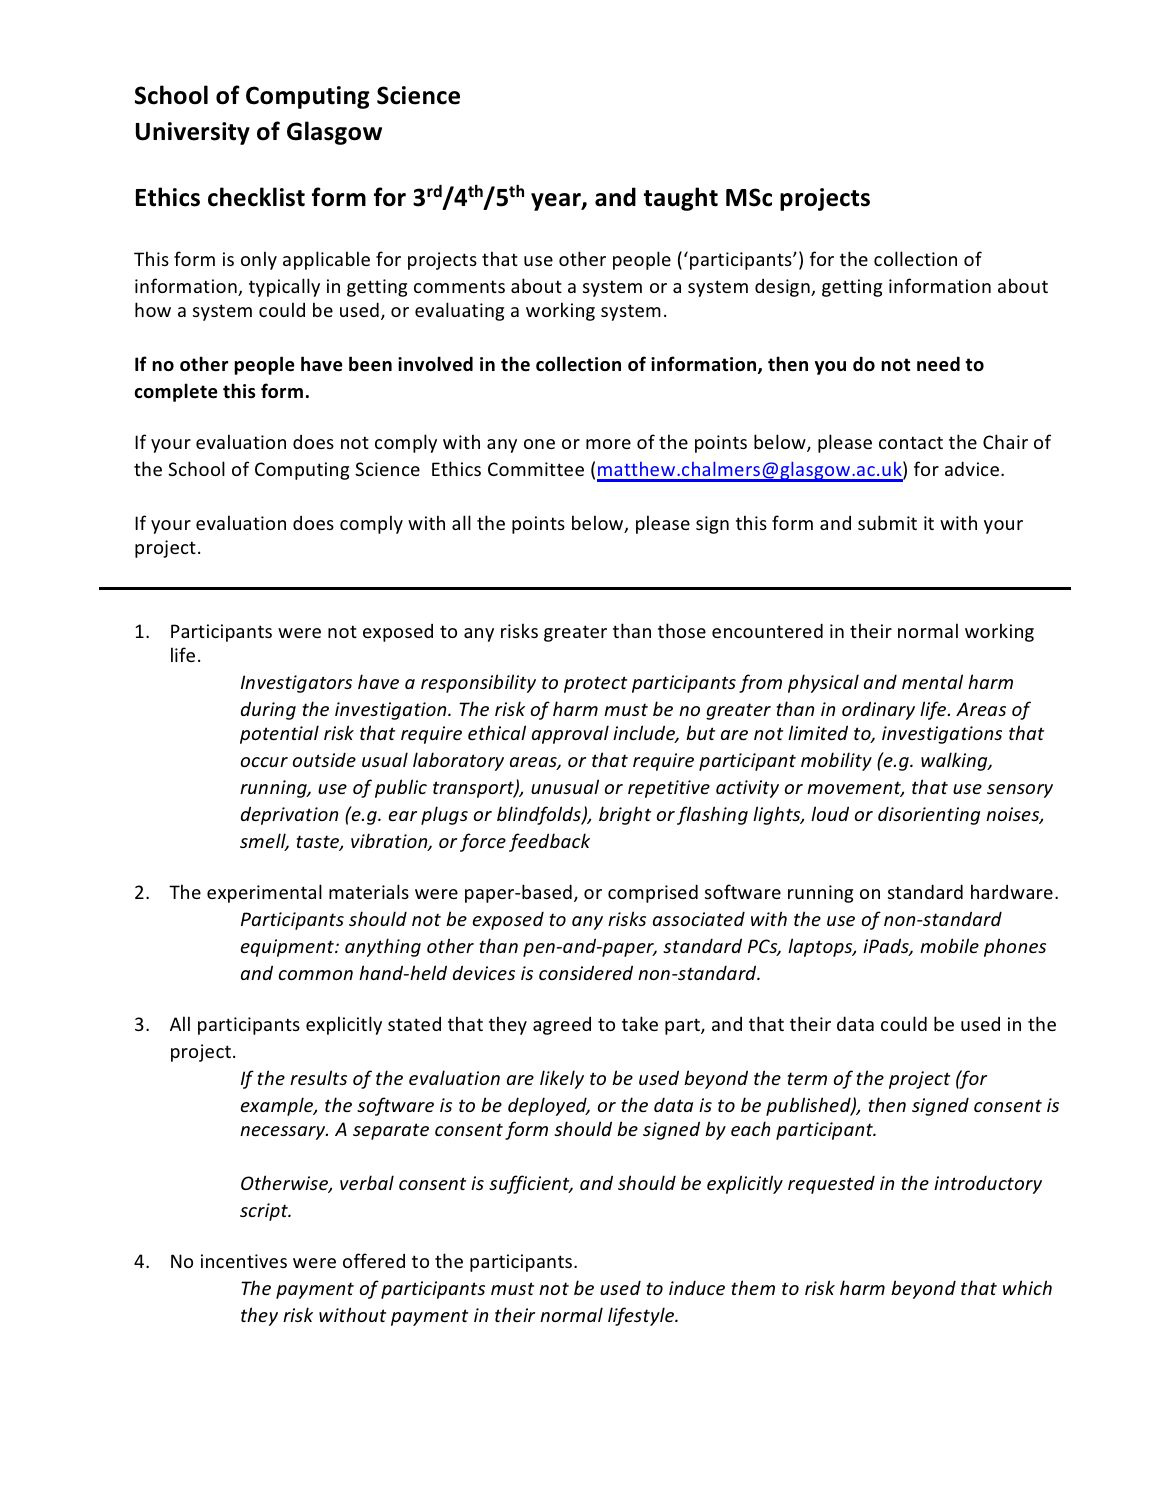
\includegraphics[width=4.70in]{ethics1}
\caption{
        }
\end{figure}




\begin{figure}[!ht]
\centering
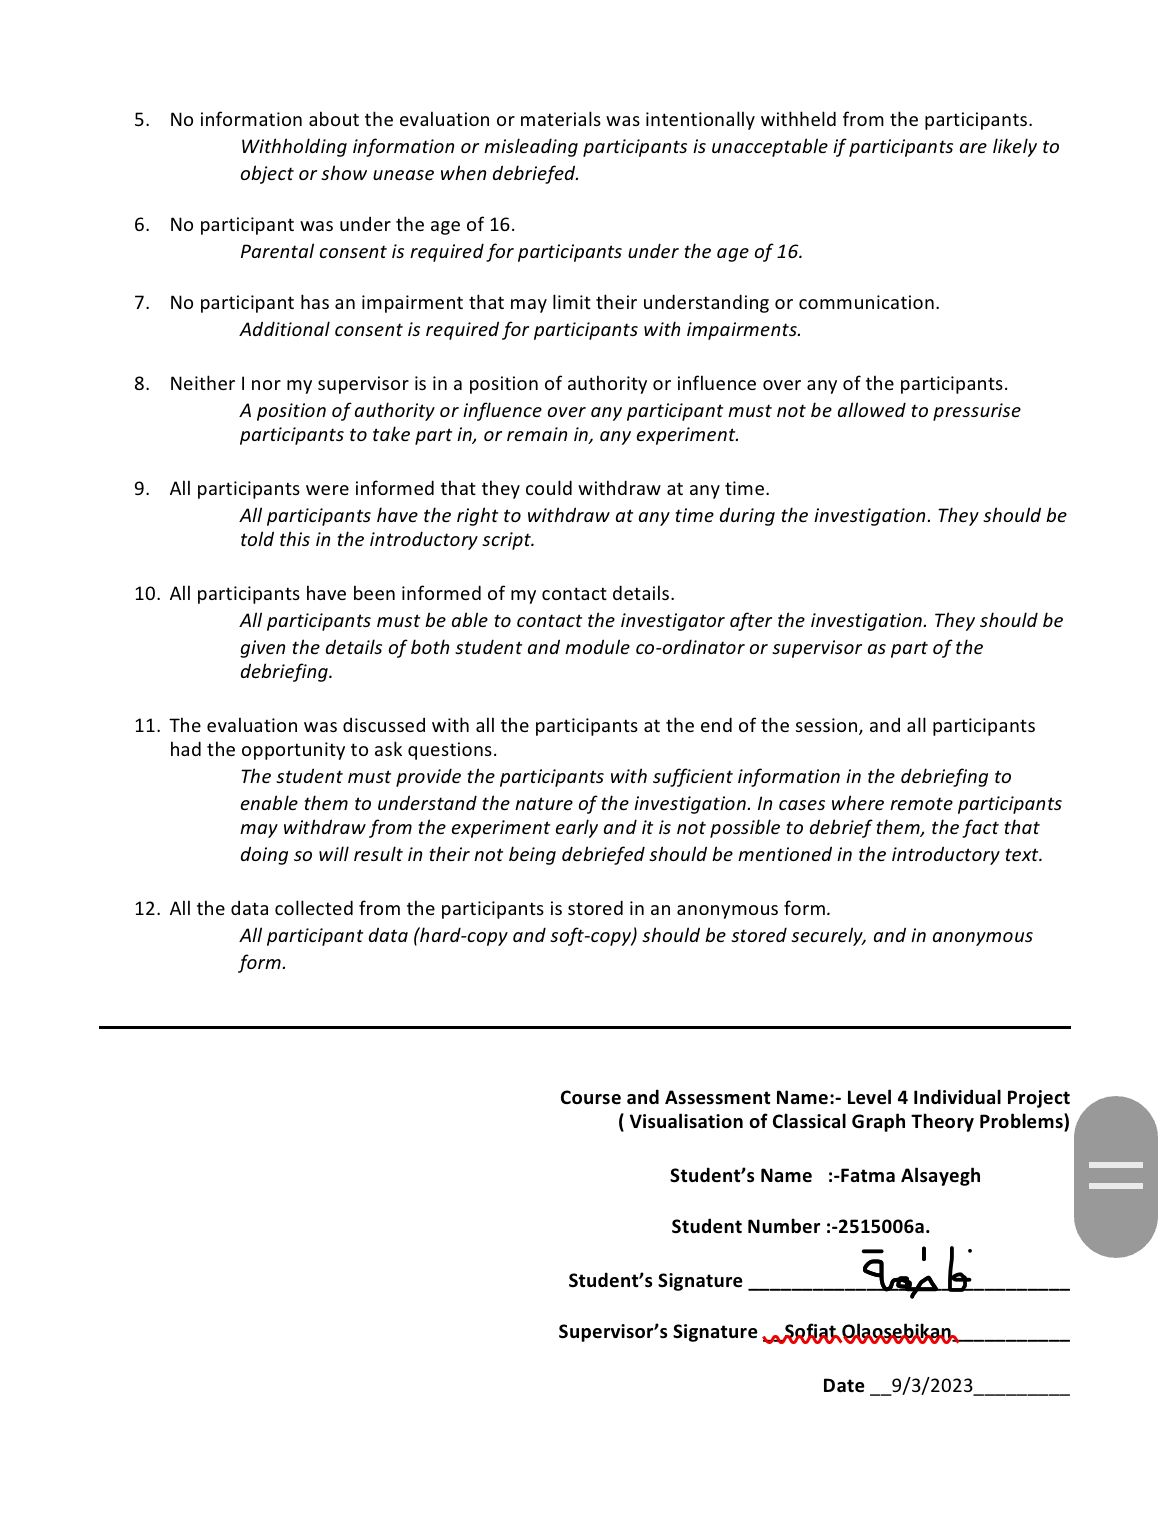
\includegraphics[width=4.70in]{ethics2}
\caption{
        }
\end{figure}

\end{appendices}

%==================================================================================================================================
%   BIBLIOGRAPHY   

% The bibliography style is abbrvnat
% The bibliography always appears last, after the appendices.

\bibliographystyle{abbrvnat}

\bibliography{l4proj}

\end{document}
